\clearpage
\appendix
\setcounter{section}{0}
\renewcommand{\thesection}{\Alph{section}}
\renewcommand{\thesubsection}{\Alph{section}.\arabic{subsection}}
\setcounter{table}{0}
\renewcommand{\thetable}{A\arabic{table}}
\setcounter{grafico}{0}
\renewcommand{\thegrafico}{A\arabic{grafico}}

\section{Estatísticas Descritivas Complementares e Testes Adicionais}
\label{ap:complementos}

\subsection{Séries produtivas, cobertura amostral e aptidão por bioma}
\label{ap:descritiva}

Este apêndice reúne os elementos descritivos complementares referidos na Seção~\ref{sec:contexto-dados}: evolução municipal das lavouras de soja e milho (Gráfico~\ref{fig:h1-lavouras}), evolução da pecuária bovina e das exportações registradas por domicílio fiscal (Tabela~\ref{tab:h1-oferta-contexto} e Gráfico~\ref{fig:h1-exportacoes}), cobertura territorial por bioma predominante (Tabela~\ref{tab:h1-cobertura}), dispersão municipal das taxas médias de conversão (Gráfico~\ref{fig:h1-distribuicao}) e distribuição do rendimento potencial GAEZ v4 (Tabela~\ref{tab:h1-capacidade}).

\begin{grafico}[htbp]
    \centering
    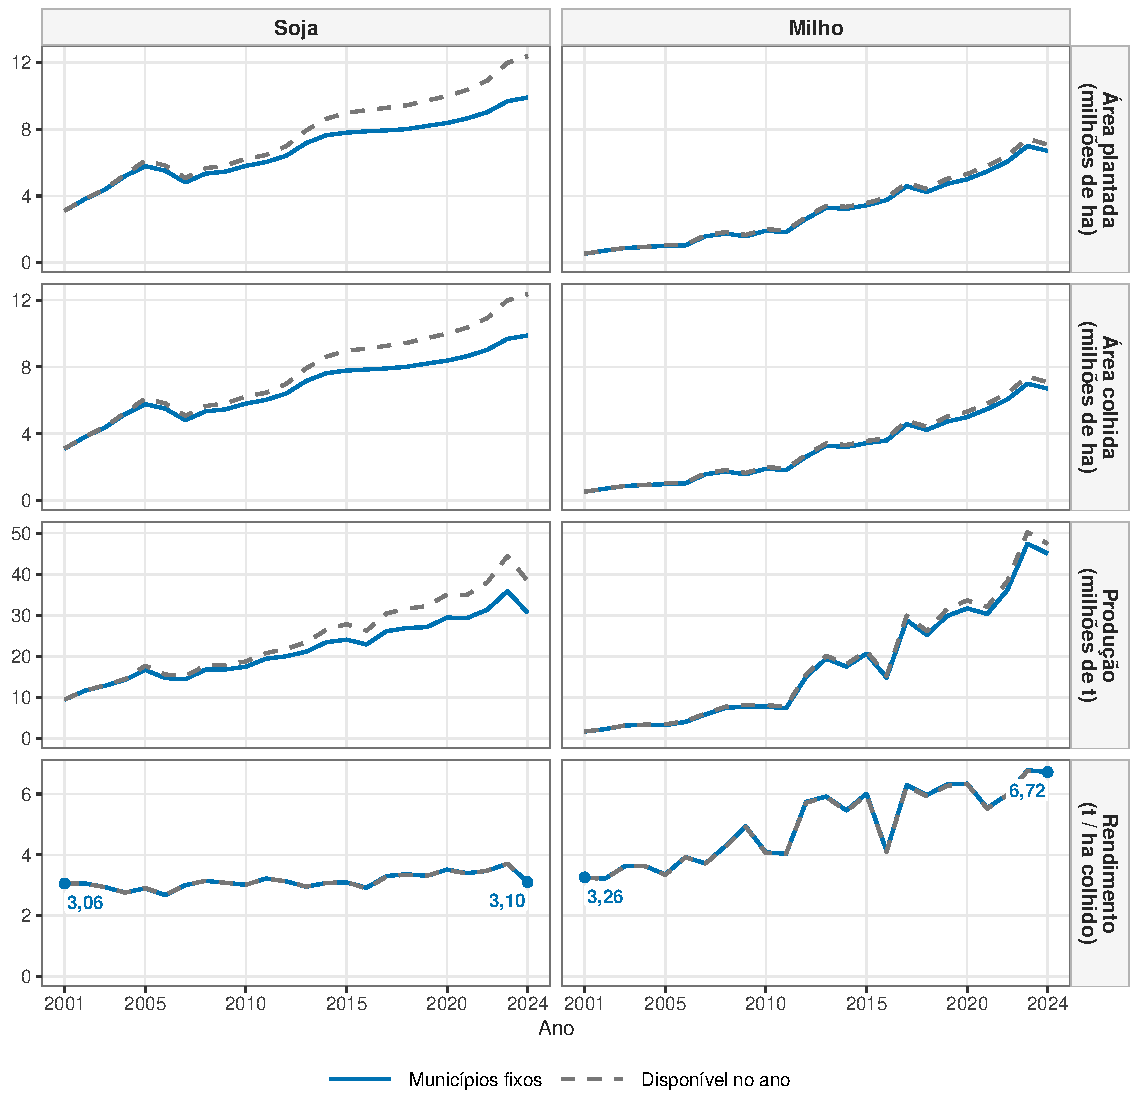
\includegraphics[width=\textwidth]{../stats/figuras/fig05_lavouras.pdf}
    \caption{Evolução das lavouras de soja e milho em Mato Grosso, 2001--2024}
    \label{fig:h1-lavouras}
    \begin{minipage}{\textwidth}\footnotesize
    \centering
    Fonte: elaboração própria, com base em IBGE/PAM.
    \end{minipage}
\end{grafico}
\FloatBarrier

\begin{table}[htbp]
\centering
\footnotesize
\captionstyle{\centering}
\normalcaption
\caption{Evolução da pecuária bovina e das exportações registradas por domicílio fiscal em Mato Grosso, 2001 e 2024}
\label{tab:h1-oferta-contexto}
\begin{tabular}{lrr}
\toprule
Indicador & 2001 & 2024 \\
\midrule
\multicolumn{3}{l}{\textit{Pecuária}} \\
Rebanho (milhões de cabeças) & 19,92 & 32,77 \\
Abate sob inspeção (milhões de cabeças) & 2,06 & 7,14 \\
Peso de carcaças (milhões de t) & 0,51 & 1,96 \\
\midrule
\multicolumn{3}{l}{\textit{Exportações FOB (US\$ milhões correntes)}} \\
Soja & 503,67 & 9.879,09 \\
Milho & 0,21 & 5.092,68 \\
Carne bovina & 5,67 & 2.308,26 \\
\bottomrule
\end{tabular}
\par\smallskip\begin{minipage}{\textwidth}\footnotesize
\centering
Fontes: IBGE/PPM; IBGE, Pesquisa Trimestral do Abate; MDIC/SECEX, Comex Stat.
\end{minipage}
\end{table}

\FloatBarrier

\begin{grafico}[htbp]
    \centering
    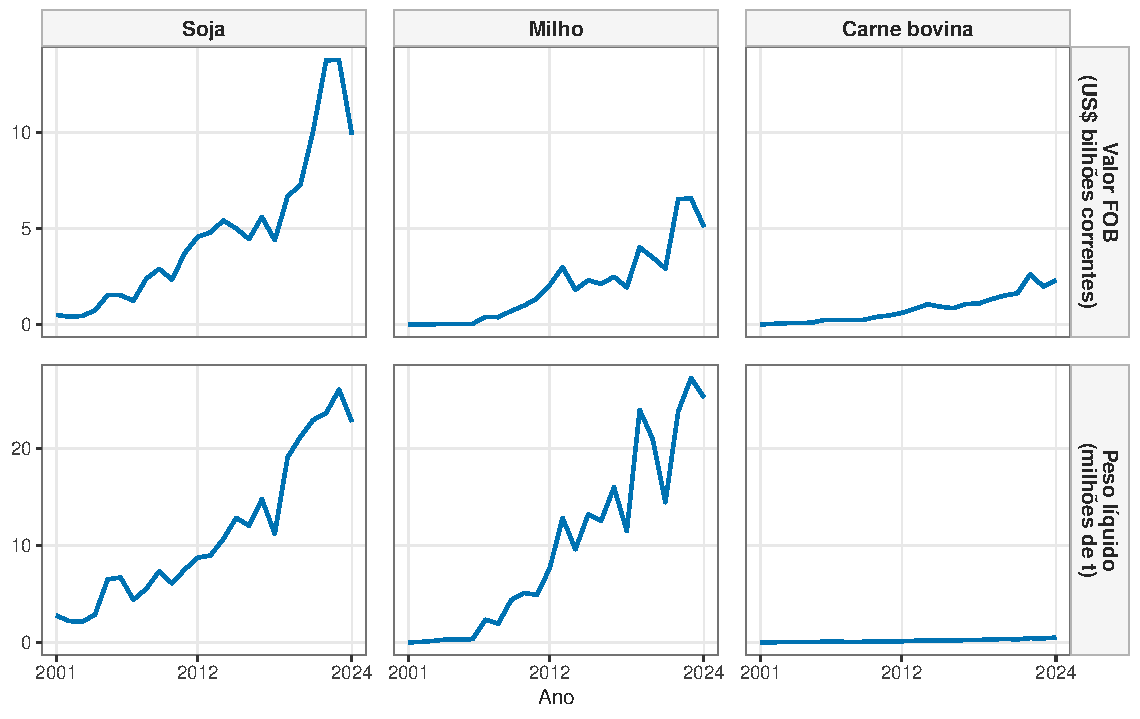
\includegraphics[width=\textwidth]{../stats/figuras/fig09_exportacoes.pdf}
    \caption{Valor e peso líquido das exportações registradas por domicílio fiscal em Mato Grosso}
    \label{fig:h1-exportacoes}
    \begin{minipage}{\textwidth}\footnotesize
    \centering
    Fonte: elaboração própria com MDIC/SECEX, Comex Stat.
    \end{minipage}
\end{grafico}
\FloatBarrier

\begin{table}[htbp]
\centering
\footnotesize
\captionstyle{\centering}
\normalcaption
\caption{Cobertura da conversão por predominância territorial, 2001--2024}\label{tab:h1-cobertura}
\begin{tabular}{lrrrrr}
\toprule
Grupo & Municípios & Mistos & Pares válidos & \% da grade & Fixos \\
\midrule
Amazônia & 76 & 35 & 1.306 & 71,6 & 39 \\
Cerrado & 61 & 24 & 1.412 & 96,4 & 55 \\
Pantanal & 4 & 4 & 54 & 56,2 & 1 \\
\bottomrule
\end{tabular}
\par\smallskip\begin{minipage}{\textwidth}\footnotesize
\SingleSpacing
\noindent\textbf{Fonte:} elaboração própria com MapBiomas 10.1 e IBGE.\par\medskip
\noindent\textbf{Nota:} Os 141 municípios (grade teórica de 3.384 pares em 24 anos) agrupam-se pelo bioma predominante; ``Mistos'' indica municípios que abrangem mais de um bioma (63). O Cerrado alcança 96,4\% de cobertura livre de nuvens (55 dos 95 municípios contínuos em ``Fixos''), contra 71,6\% na Amazônia e 56,2\% no Pantanal; as regressões retêm 2.767 dos 2.772 pares válidos após excluir grupos unitários.
\end{minipage}
\end{table}

\FloatBarrier

\begin{grafico}[htbp]
    \centering
    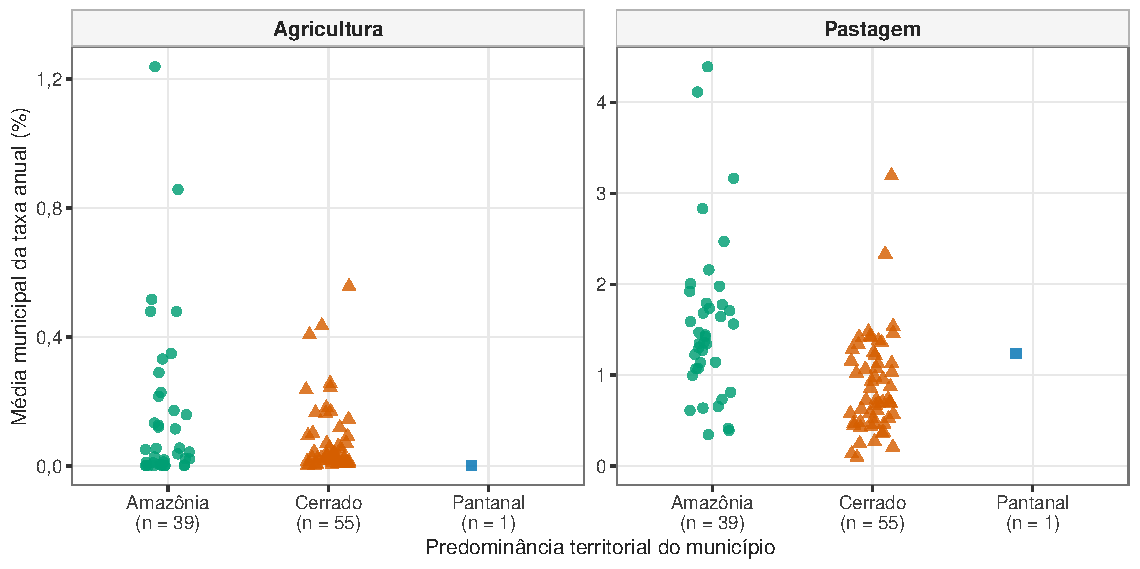
\includegraphics[width=\textwidth]{../stats/figuras/fig02_distribuicao.pdf}
    \caption{Heterogeneidade das taxas médias municipais de conversão, 2001--2024}
    \label{fig:h1-distribuicao}
    \begin{minipage}{\textwidth}\footnotesize
    \centering
    Fonte: elaboração própria com MapBiomas 10.1 e IBGE.
    \end{minipage}
\end{grafico}
\FloatBarrier

\begin{table}[htbp]
\centering
\footnotesize
\captionstyle{\centering}
\normalcaption
\caption{Rendimento potencial municipal no cenário de alto insumo e sequeiro}\label{tab:h1-capacidade}
\begin{tabular}{llrrr}
\toprule
Cultura & Predominância & Municípios & Mediana & P25--P75 \\
\midrule
Milho & Amazônia & 76 & 3.002 & 2.862--3.264 \\
Milho & Cerrado & 61 & 3.320 & 2.797--3.572 \\
Milho & Pantanal & 4 & 6.790 & 6.321--6.933 \\
Soja & Amazônia & 76 & 2.701 & 2.557--2.852 \\
Soja & Cerrado & 61 & 3.261 & 2.817--3.390 \\
Soja & Pantanal & 4 & 3.421 & 3.386--3.457 \\
\bottomrule
\end{tabular}
\par\smallskip\begin{minipage}{\textwidth}\footnotesize
\centering
Fonte: elaboração própria com FAO/IIASA, GAEZ v4, e IBGE.
\end{minipage}
\end{table}

\FloatBarrier

\subsection{Modelos complementares de pecuária, sensibilidade institucional e multiplicidade}
\label{ap:econometria}

A Tabela~\ref{tab:ap-pecuaria} reporta as estimações para conversão em pastagem e agricultura incorporando o preço real da carne bovina e a razão relativa \textit{crop-to-beef}. A Tabela~\ref{tab:ap-h1b-sens} apresenta a comparação pareada entre autos de infração de Flora e embargos ambientais na subamostra fiscal comum ($N = 1.125$), bem como os testes com conversão defasada ($Y_{i,t-1}$) e embargos futuros ($E_{i,t+1}$). Por fim, a Tabela~\ref{tab:ap-inferencia-holm} reporta os estimadores alternativos de covariância (cluster duplo, FWL-HAC e Driscoll--Kraay), o painel balanceado ($N = 2.256$), o contraste empilhado entre destinos ($N = 5.534$) e os $p$-valores ajustados pelo procedimento de Holm--Bonferroni nas famílias de testes F1 a F4.

\begin{table}[htbp]
\centering
\footnotesize
\setlength{\tabcolsep}{2.0pt}
\captionstyle{\centering}
\normalcaption
\caption{Conversão para pastagem e agricultura sob preços da carne bovina e razão \textit{crop-to-beef}, 2001--2024}
\label{tab:ap-pecuaria}
\begin{tabular}{lccccccc}
\toprule
 & (1) & (2) & (3) & (4) & (5) & (6) & (7) \\
Variável & Boi$\times H$ & Boi$\times Z$ & Pas S/B & Pas S+B & Pas M+B & Agr S/B & Agr S+B \\
\midrule
$\ln P_{c,t-1} \times Z_{i,c}$ & -- & -- & -- & 0,3963*** & 0,5810*** & -- & 0,0655** \\
 &  &  &  & (0,1321) & (0,1629) &  & (0,0293) \\
$\ln P_{\text{boi}} \times H_i^{\text{past}}$ & -0,0022 & -- & -- & -- & -- & -- & -- \\
 & (0,1711) &  &  &  &  &  &  \\
$\ln P_{\text{boi}} \times Z_{i,c}$ & -- & 0,0040 & -- & -0,3413 & -0,6503*** & -- & 0,0872** \\
 &  & (0,1590) &  & (0,2229) & (0,2436) &  & (0,0424) \\
$\ln(P_{s}/P_{\text{boi}}) \times Z_{i,s}$ & -- & -- & 0,3941*** & -- & -- & 0,0593** & -- \\
 &  &  & (0,1335) &  &  & (0,0270) &  \\
$H_i^{\text{past}} \times \tau_t$ & 0,0917 & -- & -- & -- & -- & -- & -- \\
 & (0,0630) &  &  &  &  &  &  \\
$Z_{i,c} \times \tau_t$ & -- & 0,0057 & 0,0295 & 0,0170 & 0,1303** & 0,0585*** & 0,0238** \\
 &  & (0,0508) & (0,0496) & (0,0534) & (0,0580) & (0,0212) & (0,0114) \\
Precipitação ($R_{it}$) & -0,0158 & -0,0216 & -0,0225 & -0,0227 & -0,0194 & -0,0131** & -0,0137** \\
 & (0,0147) & (0,0156) & (0,0155) & (0,0157) & (0,0156) & (0,0061) & (0,0063) \\
\midrule
Observações & 2.767 & 2.767 & 2.767 & 2.767 & 2.767 & 2.767 & 2.767 \\
$R^2$ total & 0,4919 & 0,4900 & 0,4918 & 0,4919 & 0,4945 & 0,3819 & 0,3831 \\
$R^2$ \textit{within} & 0,0046 & 0,0009 & 0,0046 & 0,0046 & 0,0098 & 0,0183 & 0,0203 \\
EF Mun. + Bioma$\times$Ano & Sim & Sim & Sim & Sim & Sim & Sim & Sim \\
\bottomrule
\end{tabular}
\par\smallskip\begin{minipage}{\textwidth}\footnotesize
\SingleSpacing
\noindent\textbf{Fonte:} elaboração própria com MapBiomas 10.1, Banco Mundial, BLS/FRED, FAO/IIASA (GAEZ v4) e IBGE.\par\medskip
\noindent\textbf{Nota:} As colunas (1)--(5) adotam como variável dependente a conversão bruta para pastagem (p.p.) e (6)--(7) para agricultura ($N = 2.767$). O preço da carne bovina isolado (1--2) não apresenta associação estatística com a abertura de pastos, enquanto preços de grãos e a razão soja/boi (\textit{crop-to-beef}) exibem associação positiva em (3--5), compatível com conversão voltada à valorização agrícola futura. Erros-padrão por município (* $p<0{,}10$; ** $p<0{,}05$; *** $p<0{,}01$).
\end{minipage}
\end{table}

\FloatBarrier

\begin{table}[htbp]
\centering
\footnotesize
\setlength{\tabcolsep}{2.4pt}
\captionstyle{\centering}
\normalcaption
\caption{Ponte na subamostra fiscal alinhada ($N=1.125$) e testes de sensibilidade à focalização dos embargos}
\label{tab:ap-h1b-sens}
\begin{tabular}{lccccc}
\toprule
 & (1) & (2) & (3) & (4) & (5) \\
\multicolumn{6}{l}{\textit{Painel A: Subamostra fiscal comum (Soja, $N = 1.125$)}} \\
Variável & Base & Autos M6 & Autos M7 & Área Emb. & Mod. Emb. \\
\midrule
$\ln P_{s,t-1} \times Z_{i,s}$ & 0,0230 & 0,0225 & 0,0439 & 0,0109 & 0,0150 \\
 & (0,0544) & (0,0544) & (0,0724) & (0,0601) & (0,0669) \\
Autos / Emb. ($t-1$) & -- & 0,0034 & -0,0009 & -0,0030 & 0,0030 \\
 &  & (0,0063) & (0,0059) & (0,0026) & (0,0067) \\
Tripla ($\ln P \times Z \times \text{Inst}$) & -- & -- & -0,0062 & -- & 0,0112 \\
 &  &  & (0,0121) &  & (0,0152) \\
$Z_{i,s} \times \tau_t$ & 0,0143 & 0,0146 & 0,0129 & 0,0159 & 0,0168 \\
 & (0,0235) & (0,0234) & (0,0228) & (0,0232) & (0,0204) \\
Observações (Painel A) & 1.125 & 1.125 & 1.125 & 1.125 & 1.125 \\
$R^2$ \textit{within} (Painel A) & 0,0046 & 0,0048 & 0,0089 & 0,0065 & 0,0076 \\
\midrule
\multicolumn{6}{l}{\textit{Painel B: Dinâmica ($Y_{i,t-1}$) e placebo ($E_{i,t+1}$)}} \\
Variável & Dyn. Ár. (S) & Dyn. Ár. (M) & Dyn. Mod. & Lead Ár. & Lead Mod. \\
\midrule
$\ln P_{c,t-1} \times Z_{i,c}$ & 0,0400** & 0,0097 & 0,0484** & 0,0804** & 0,0906** \\
 & (0,0199) & (0,0068) & (0,0206) & (0,0355) & (0,0387) \\
Embargos ($t-1$) & -0,0028* & -0,0030* & 0,0067 & -0,0072** & 0,0077 \\
 & (0,0017) & (0,0017) & (0,0085) & (0,0029) & (0,0124) \\
Tripla ($t-1$) & -0,0001 & 0,0062 & -0,0207 & -0,0006 & -0,0251 \\
 & (0,0050) & (0,0053) & (0,0153) & (0,0096) & (0,0378) \\
Conversão ($Y_{i,t-1}^{\text{agr}}$) & 0,5487*** & 0,5495*** & 0,5491*** & -- & -- \\
 & (0,0276) & (0,0279) & (0,0274) &  &  \\
Embargos futuros ($t+1$) & -- & -- & -- & -0,0026 & 0,0017 \\
 &  &  &  & (0,0035) & (0,0147) \\
Tripla futura ($t+1$) & -- & -- & -- & -- & -0,0108 \\
 &  &  &  &  & (0,0381) \\
\midrule
Observações (Painel B) & 2.590 & 2.590 & 2.590 & 2.633 & 2.633 \\
$R^2$ \textit{within} (Painel B) & 0,3432 & 0,3429 & 0,3433 & 0,0208 & 0,0200 \\
EF Mun. + Bioma$\times$Ano & Sim & Sim & Sim & Sim & Sim \\
\bottomrule
\end{tabular}
\par\smallskip\begin{minipage}{\textwidth}\footnotesize
\SingleSpacing
\noindent\textbf{Fonte:} elaboração própria com MapBiomas 10.1, IBAMA e FAO/IIASA (GAEZ v4). Todos os termos inferiores das triplas incluídos.\par\medskip
\noindent\textbf{Nota:} Variável dependente em p.p. ($Y_{mt}^{\text{agr}}$). No Painel A ($N = 1.125$), restrito aos pares com autuações de Flora tematicamente completas, nem autos nem embargos (tampouco $\ln P \times Z$) atingem significância estatística. No Painel B, a área embargada defasada mantém sinal negativo a 10\% com controle dinâmico $Y_{i,t-1}$ (1--2) e a 5\% diante do placebo futuro em $t+1$ (4), enquanto as interações triplas perdem precisão. Erros-padrão por município (* $p<0{,}10$; ** $p<0{,}05$; *** $p<0{,}01$).
\end{minipage}
\end{table}

\FloatBarrier

\begin{table}[htbp]
\centering
\footnotesize
\setlength{\tabcolsep}{3.0pt}
\captionstyle{\centering}
\normalcaption
\caption{Inferência alternativa, painel balanceado, contraste entre destinos e ajuste de Holm--Bonferroni}
\label{tab:ap-inferencia-holm}
\begin{tabular}{lcccc}
\toprule
\multicolumn{5}{l}{\textit{Painel A: Inferência alternativa, painel balanceado e contraste Agr. $-$ Past.}} \\
Especificação / Covariância & Est. (Soja) & $p$ (S) & Est. (Milho) & $p$ (M) \\
\midrule
Ref. (Cluster Mun., $G=134$) & 0,0848** (0,0358) & 0,0192 & 0,0519*** (0,0179) & 0,0043 \\
Cluster Duplo (Mun. + Ano) & 0,0848* (0,0481) & 0,0909 & 0,0519* (0,0277) & 0,0741 \\
FWL-HAC (24 escores, lag 2) & 0,0848** (0,0360) & 0,0274 & 0,0519* (0,0252) & 0,0509 \\
Driscoll--Kraay (lag 2) & 0,0848** (0,0382) & 0,0366 & 0,0519* (0,0267) & 0,0647 \\
Painel balanceado ($N=2.256$) & 0,0827** (0,0400) & 0,0413 & 0,0543*** (0,0206) & 0,0098 \\
Empilhada Agr. $-$ Past. ($N=5.534$) & -0,2357** (0,0952) & 0,0145 & -0,4081*** (0,1369) & 0,0034 \\
\midrule
\multicolumn{5}{l}{\textit{Painel B: Correção de multiplicidade de Holm--Bonferroni por família de testes}} \\
Família / Hipótese Testada & Estimativa & EP & $p$ bruto & $p_{\text{Holm}}$ \\
\midrule
\multicolumn{5}{l}{\textbf{F1: H1a e Biomas ($m=6$)}} \\
\quad M1 Soja MT & 0,0848* & (0,0358) & 0,0192 & 0,0767 \\
\quad M2 Milho MT & 0,0519** & (0,0179) & 0,0043 & 0,0248 \\
\quad Soja Amazônia & 0,0866 & (0,0610) & 0,1597 & 0,3194 \\
\quad Soja Cerrado & 0,0752 & (0,0439) & 0,0920 & 0,2759 \\
\quad Milho Amazônia & 0,0185 & (0,0514) & 0,7197 & 0,7197 \\
\quad Milho Cerrado & 0,0572** & (0,0192) & 0,0041 & 0,0248 \\
\multicolumn{5}{l}{\textbf{F2: H1b Instituições ($m=6$)}} \\
\quad Área embargada (Soja) & -0,0076** & (0,0029) & 0,0091 & 0,0454 \\
\quad Área embargada (Milho) & -0,0082** & (0,0030) & 0,0068 & 0,0407 \\
\quad Tripla N embargos (Soja) & -0,0314 & (0,0179) & 0,0810 & 0,3242 \\
\quad Tripla N embargos (Milho) & 0,0068 & (0,0165) & 0,6828 & 1,0000 \\
\quad Autos alinhado (Soja, $N=1.125$) & 0,0034 & (0,0063) & 0,5896 & 1,0000 \\
\quad Tripla autos alinhado (Soja) & -0,0062 & (0,0121) & 0,6084 & 1,0000 \\
\multicolumn{5}{l}{\textbf{F3: Regimes 06--11 e Destinos ($m=6$)}} \\
\quad Painel A Amazônia 2006--11 (Soja) & -0,0643 & (0,0318) & 0,0471 & 0,1247 \\
\quad Painel A Cerrado 2006--11 (Soja) & 0,0523 & (0,0250) & 0,0402 & 0,1247 \\
\quad Painel B Amazônia 2006--11 (Soja) & -0,0704 & (0,0334) & 0,0384 & 0,1247 \\
\quad Painel B Cerrado 2006--11 (Soja) & 0,0569 & (0,0258) & 0,0312 & 0,1247 \\
\quad Empilhado Agr. $-$ Past. (Soja) & -0,2357* & (0,0952) & 0,0145 & 0,0727 \\
\quad Empilhado Agr. $-$ Past. (Milho) & -0,4081** & (0,1369) & 0,0034 & 0,0205 \\
\multicolumn{5}{l}{\textbf{F4: Pecuária / Pastagem ($m=7$)}} \\
\quad Pastagem: Boi $\times H^{\text{past}}$ & -0,0022 & (0,1711) & 0,9897 & 1,0000 \\
\quad Pastagem: Boi $\times$ GAEZ & 0,0040 & (0,1590) & 0,9798 & 1,0000 \\
\quad Pastagem: Razão Soja/Boi $\times$ GAEZ & 0,3941** & (0,1335) & 0,0037 & 0,0161 \\
\quad Pastagem conjunta: Soja $\times$ GAEZ & 0,3963** & (0,1321) & 0,0032 & 0,0161 \\
\quad Pastagem conjunta: Boi $\times$ GAEZ & -0,3413 & (0,2229) & 0,1281 & 0,3843 \\
\quad Pastagem: Soja $\times$ GAEZ & 0,3206** & (0,1016) & 0,0020 & 0,0119 \\
\quad Pastagem: Milho $\times$ GAEZ & 0,4600*** & (0,1397) & 0,0013 & 0,0089 \\
\bottomrule
\end{tabular}
\par\smallskip\begin{minipage}{\textwidth}\footnotesize
\SingleSpacing
\noindent\textbf{Fonte:} elaboração própria. Asteriscos no Painel B indicam significância após ajuste de Holm--Bonferroni (* $p_{\text{Holm}}<0{,}10$; ** $p_{\text{Holm}}<0{,}05$; *** $p_{\text{Holm}}<0{,}01$).\par\medskip
\noindent\textbf{Nota:} No Painel A (asteriscos pelo $p$-valor bruto), soja e milho mantêm significância a 10\% ou menos sob covariâncias conservadoras e no painel contínuo ($N = 2.256$), enquanto o modelo empilhado aponta menor resposta na agricultura que na pastagem. No Painel B, o ajuste de Holm--Bonferroni preserva os efeitos principais (F1, F2 área embargada, F3 destinos e F4 \textit{crop-to-beef}), elevando os contrastes de 2006--2011 para $p_{\text{Holm}} = 0{,}1247$, sem comprovar nulidade.
\end{minipage}
\end{table}

\FloatBarrier
